\section{Applying the C2W model}

\subsection{Language Modeling}
\label{subsec:language-model-c2w}

In this section we use the C2W model and a recurrent LSTM to perform language modeling as 
described in~\cite{DBLP:journals/corr/LingLMAADBT15}.
The neural network is going to compute the log propability $\log[ p(\mathcal{w}) ]$ of the 
sentence $\mathcal{w} = (w_1, \dots, w_m)$. As previously discussed in section~\ref{sec:language-modeling} this can be 
decomposed into the sum of the conditional log probabilities $log[ p(w_1,\dots,w_m) ] = \sum_{i=1}^{m} log[ p(w_i | w_1,\dots,w_{i-1}) ]$.
This model will compose the previously described word representations of $w_1,\dots,w_{i-1}$ to compute 
$log[ p(w_i | w_1,\dots,w_{i-1}) ]$ using a LSTM unit.
The model is shown in figure~\ref{fig:c2w-language-model}. The first stage can use either the embeddings generated with the C2W model
$f(w_i) = e_{w_i}^C $ or simply word lookup tables $e_{w_i}^W = P * 1_{w_i}$.

Every time we input a new word $w_i$ from the sequence we get the LSTM state $s_i$. The state $s_i$ is then used to predict word $w_{i+1}$.
The state $s_i$ is projected into a vector of size $|V|$ (the vocabulary size). The softmax is a $d \times V$ table, 
which encodes the likelihood of every word type in the vocabulary in a given context. 
The softmax layer will ensure a valid log probability distribution. This way we can choose the word type with the maximal likelihood.
Maximizing the conditional log-likelihoods during training will improve the modeling 
of $p(\mathcal{w})$~\cite{DBLP:conf/interspeech/MikolovKBCK10}.
More details regarding the softmax layer are explained in section~\ref{subsec:softmax}.

\begin{figure}[H]
\begin{center}
  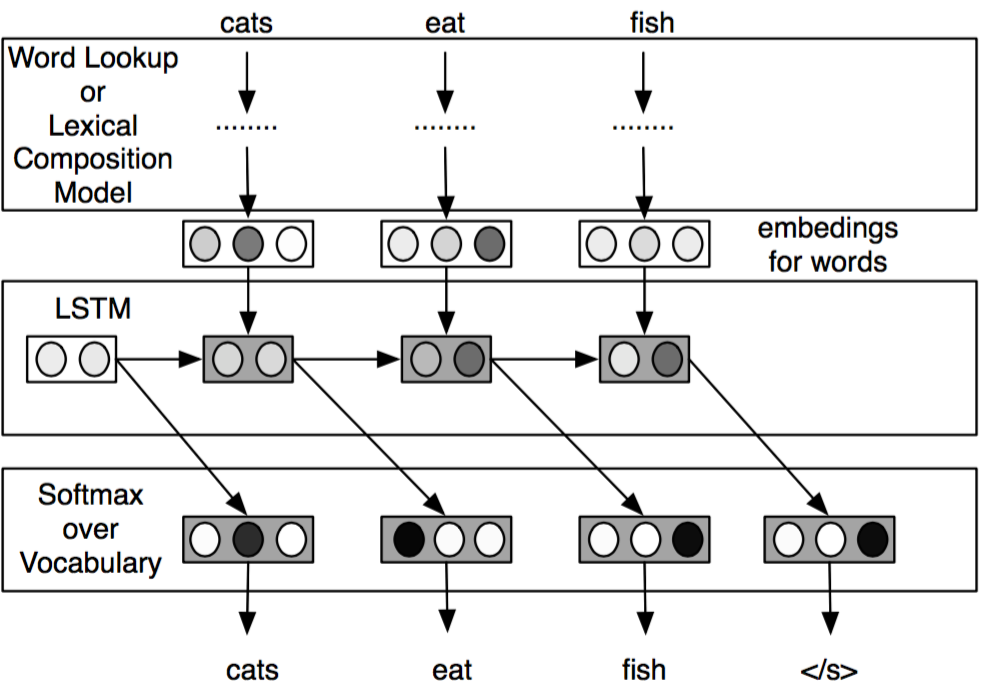
\includegraphics[width=0.6\textwidth]{./img/c2w-language-model}
  \caption{Neural network for language model. The C2W model is at the top, the word embeddings are then fed into an recurrent LSTM.
  Finally }
  \label{fig:c2w-language-model}
\end{center}
\end{figure}


\subsubsection{Evaluation}

In the orginal paper~\cite{DBLP:journals/corr/LingLMAADBT15}, the perplexity~\ref{subsec:perplexity} is 
used to evaluate the performance of the language model with different configurations. 
However the perplexity cannot be used to compare models with different vocabularies,
since there are fewer outcomes in the softmax, the global perplexity can decrease.

% ==========================================================================================
% \subsection{Part-of-Speech Tagging}


% ==========================================================================================
\subsection{Morphological inflection generation}

Another application of C2W like model beyond language modeling is the morphological inflection generation~\cite{DBLP:journals/corr/FaruquiTND15}.
The goal is to perform a lingustic transformation some examples of the inflections which this model seeks to generate can be seen in table~\ref{tab:inflections}.
First stage is the \textbf{encoder}:\\
This part of the model is eqvivalent to the C2W model: Each word $w$ is broken up into it's characters $e_{c_1}^C, \dots, e_{c_m}^C$.
Then a bidirectional LSTM layer is used and th result is composed into $e_{w}$.
Second part is the \textbf{decoder}:\\
This is a LSTM unit which will sequentially receive the word characters as input combined with the previous output and the word vector.
Every output state is computed as $s_t = g(s_{t-1}, \{e_{w}, y_{t-1}, x_t\})$. Where $g$ is the decoder LSTM unit,
$s_t$ is the LSTM output, $y_{t-1}$ the actual character output and $x_t$ is the current input character.
Since the input word might be shorter than the output, onece the input sequence runs out of characters we feed in an $\epsilon$ character
indicating null input: $x_t = \epsilon$. The vector representation for the $\epsilon$ character is learned just like in the C2W model.


\begin{figure}[H]
\begin{center}
  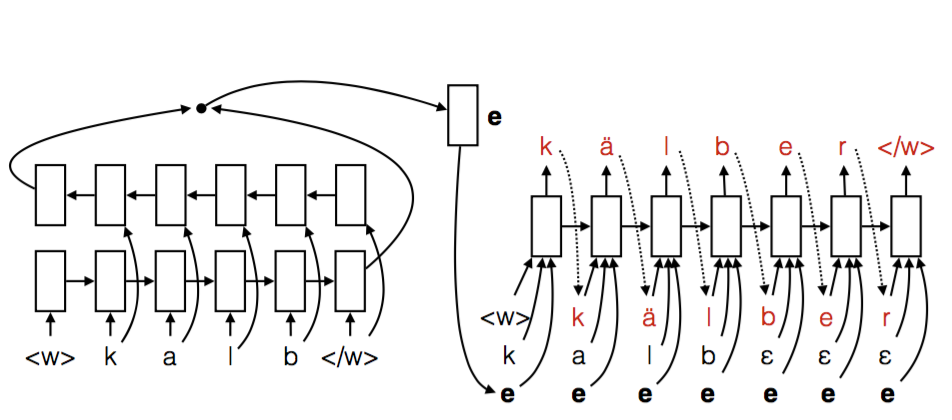
\includegraphics[width=\textwidth]{./img/inflection-generatior}
  \caption{A endoder decoder structure for inflection generation}
  \label{fig:inflection-generatior}
\end{center}
\end{figure}

\begin{table}
\begin{center}
\begin{tabular}{ l l l l }
  \hline
             & singular & plural \\ \hline
  nominative & Kalb & K\"alber \\
  accusative & Kalb & K\"alber \\
  dative & Kalb & K\"albern \\
  genitive & Kalbes & K\"alber \\
\end{tabular}
\end{center}
\caption{Example of an inflection table for the word Kalb (calf, German).}
\label{tab:inflections}
\end{table}

Converting the word embeddings from a C2W like model back into inflected versions of the word 
as discussed in Faruqui et al. \cite{DBLP:journals/corr/FaruquiTND15}

% Comparison of current LSTMs based word embeddings with the character based method from Santos et al. \cite{DBLP:conf/icml/2014}